\documentclass{beamer}
\beamertemplatenavigationsymbolsempty
\usepackage{amsmath, amssymb, hyperref, graphics}
\usepackage{tikz}

\title{Graph Theory Lecture 6}

\begin{document}
\begin{frame}{Warm-up: what's all this then?}
 \begin{figure} 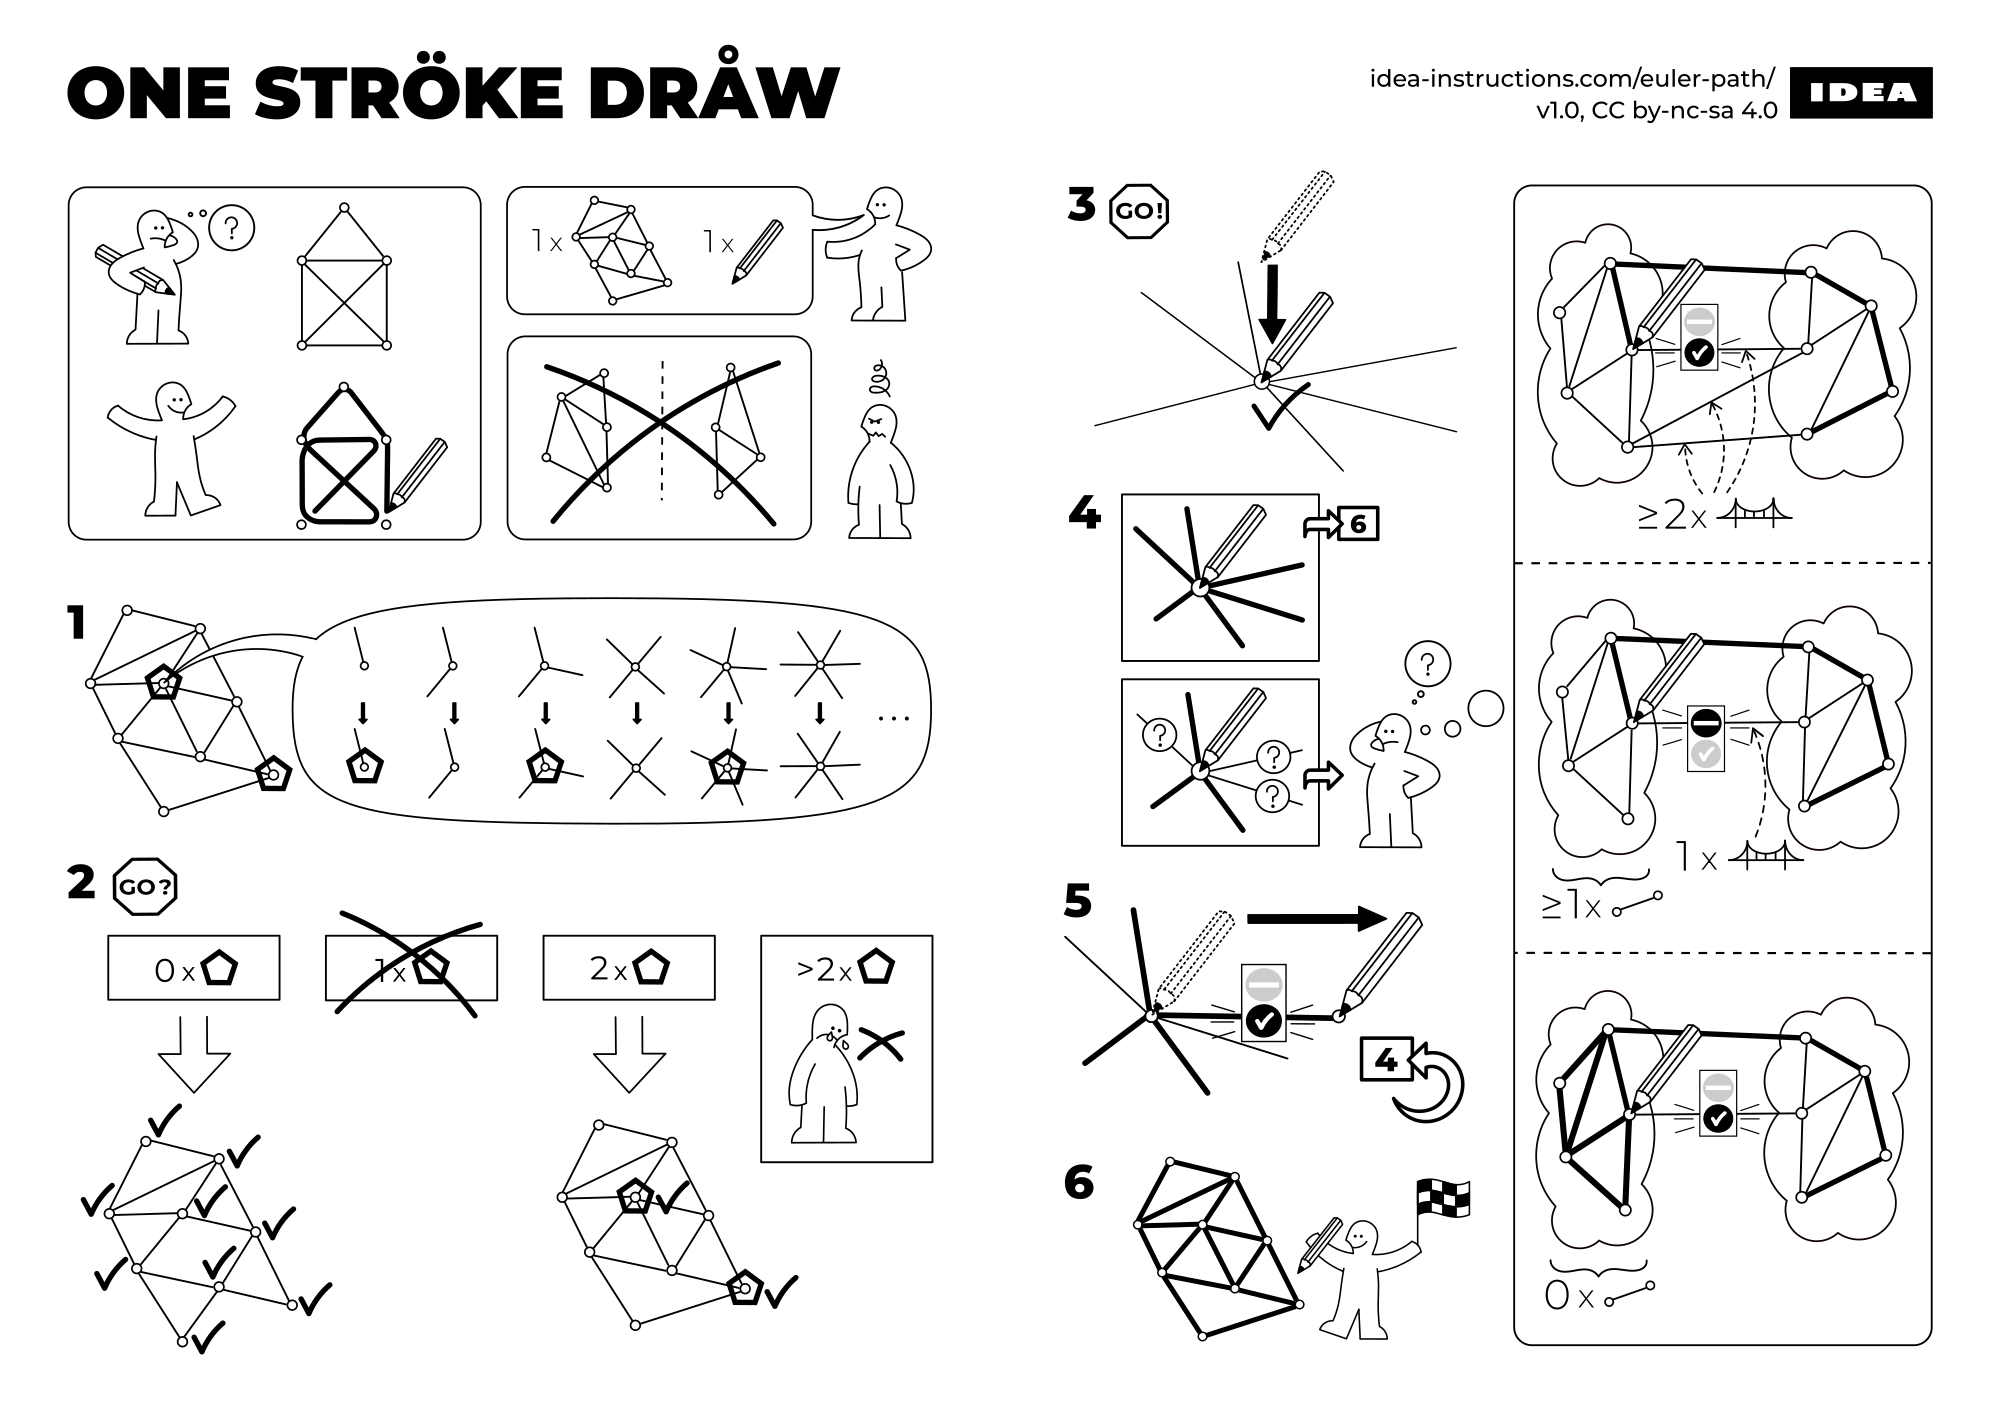
\includegraphics[width=\textwidth]{Pictures/euler-path.png}
   \caption{Fleury's algorithm for finding Hamiltonian paths/cycles}
   \end{figure}
\end{frame}  




\begin{frame}{To prove a graph is Hamiltonian, find a cycle}
   \begin{definition}A graph $G$ is \emph{Hamiltonian} if there is a closed walk that visits every vertex exactly once. $G$ is \emph{semi-Hamiltonian} if there is a not necessarily closed walk that visits every vertex exactly once.
  \end{definition}
  \begin{figure}
      \caption{The dedecahedron graph $D_{20}$ is Hamiltonian}
       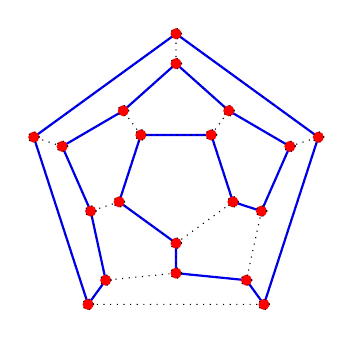
\begin{tikzpicture}[scale=.38]

 \begin{scope}[every node/.style={draw, circle, fill=red, inner sep=0pt, minimum width=4pt} ]  
   \draw[thick, blue] (-18:2)--(54:2)--(126:2)--(198:2)--(270:2)--(270:3)--(306:4)--(306:5)--(18:5)--(90:5)--(162:5)--(234:5)--(234:4)--(198:3)--(162:4)--(126:3)--(90:4)--(54:3)--(18:4)--(-18:3)--(-18:2);

   \draw[dotted] \foreach \x in {0,72,...,288}
    {
        (\x-90:2) node {}  -- (\x-18:2)
      (\x-90:2) -- (\x-90:3)
      (\x-90:3) -- (\x-54:4)
      (\x-90:3) node {} -- (\x-126:4)
      (\x+90:4) node {} -- (\x+90:5)
      (\x+90:5) node {} -- (\x+18:5)
     };
   \end{scope}
  \end{tikzpicture}
    \end{figure}

\end{frame}   

\begin{frame}{Proving a graph \emph{isn't} Hamiltonian is hard}
  \begin{block}{In \emph{theory} it's easy:}
    Only finitely many possible paths; check them all.
  \end{block}
  \begin{block}{But number of possible paths grows very quickly}
We can't prove there's no easy way to check if a graph is Hamiltonian or not, but we've bet the world economy that there isn't.
  \end{block}
  
\begin{block}{Mathematical culture: NP-completeness}
  Determining whether or not a graph is Hamiltonian is ``NP-complete'' i.e., any problem in NP can be reduced to checking whether or not a certain graph is Hamiltonian. 
\end{block}
If we found an easy algorithm, could break standard encryption.
  \end{frame}


\begin{frame}{Proving a graph isn't Hamiltonian: case-by-case}
  \begin{theorem}If we remove a vertex from $D_{20}$, it is not longer Hamiltonian.
  \end{theorem}
  \begin{block}{Proof Sketch}

    \begin{itemize}
\item Suppose $D_{20}$ was Hamiltonian
\item At every vertex, exactly two edges used in cycle
\item Suppose certain edge in cycle, chase consequences: \\
  Other edges must be in/out of cycle
\item Iterate 
    \end{itemize}
Useful observations: edges can't make a smaller cycle
    \end{proof}
This strategy will work in general, but may be very complicated.
\end{frame}

\begin{frame}{Proving $G$ isn't Hamiltonian: tricks}
  \begin{block}{Can't contain certain configurations:}
\begin{center}    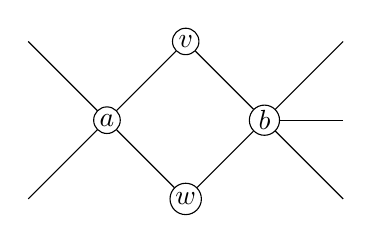
\begin{tikzpicture}[every node/.style={draw, circle, fill=white, inner sep=1pt, minimum width=6pt} ]
      \draw (-1,1)--(0,0)--(-1,-1);
      \draw (3,1)--(2,0)--(3,-1);
      \draw (3,0)--(2,0);
      \node (a) at (0,0) {$a$};
      \node (b) at (2,0) {$b$};
      \node (v) at (1,1) {$v$};
      \node (w) at (1,-1) {$w$};
\draw (a)--(v)--(b)--(w)--(a);
      \end{tikzpicture}
\end{center}
\end{block}
  \begin{lemma}If $G$ is bipartite and Hamiltonian, then $G$ has the same number of red and blue vertices.
    \end{lemma}
    \begin{proof}
      \begin{itemize}
      \item          The vertices in the Hamiltonian cycle alternate red and blue
        \item The Hamiltonian cycle contains all the vertices
\end{itemize}
      \end{proof}  

\end{frame}
\begin{frame}{Tool: assume $G$ is Hamiltonian, consider ``extra'' edges}
  \begin{theorem}The Petersen graph $P$ isn't Hamiltonian
  \end{theorem}

  \begin{proof}
    Suppose $P$ is Hamiltonian.  The Hamiltonian cycle uses up two edges at each vertex, so we have one more edge meeting each vertex.

\begin{block}{Analyze how to place these five edges.}
    \begin{itemize}
    \item Can't go to next vertex in cycle: no multiple edges
    \item Can't ``skip'' one or two: $P$ has no 3 or 4 cycles
    \item So extra edges ``straight across'' $\pm 1$ 
    \item Rule out straight across
    \item Rule out all ``skip 3''
        \end{itemize}
\end{block}
\end{proof}
\end{frame}




\begin{frame}{A sufficient condition to be Hamiltonian}
\begin{block}{If we have ``enough'' edges, should be Hamiltonian}
  If $G$ is Hamiltonian and we add extra edges, the result is still Hamiltonian.
\end{block}

\begin{theorem}[Ore] Let $G$ be a simple graph with $n$ vertices, so that for any two nonadjacent vertices $v$ and $w$, we have $deg(v)+deg(w)\geq n$.  Then $G$ is Hamiltonian.
\end{theorem}
\alert{Not an ``If and only If!'' -- won't prove $G$ isn't Hamiltonian}
\begin{block}{Proof ingredients}
  \begin{itemize}
    \item ``Minimal Criminal'': minimal/maximal counterexamples have extra structure
    \item ``adding extra edges''
    \item Pigeonhole principal
\end{itemize}
  \end{block}
\end{frame}



\begin{frame}{Proof of Ore's Theorem}
\begin{block}{Minimal criminimal:}
  Assume $G$ is a counterexample, but then adding any edge to $G$ makes it Hamiltonian.  \\ Then $G$ must be semi-Hamiltonian.
\end{block}
  \begin{block}{Adding extra edges}
  Let $v_1-v_2-\dots-v_n$ be the Hamiltonian path.  $v_1$ and $v_2$ not adjacent so $deg(v_1)+deg(v_2)\geq n$.  \\
  So we need to add $n-2$ more edges to $v$ or $w$.
\end{block}
\begin{block}{Pigeon hole principle}
  Let $i\in 3,\dots, n-1$ with $v_1$ adjacent to $v_i$ and $v_n$ adjacent to $v_{i-1}$: then we have a Hamiltonian path! \\
  Use pigeon-hole principle to find such an $i$.
  \end{block}
  \end{frame}


\end{document}
